%!BIB TS-program = 
\documentclass{beamer}
% Introdução ao LaTeX
% Seminário LaTeX -- o Livro
% Geraldo Xexéo
% Este arquivo tem a licença Creative Commons
% BY-NC-SA 2020

%\usepackage[utf8]{inputenc}
\usepackage[T1]{fontenc}
% Introdução ao LaTeX
% Seminário LaTeX -- o Livro
% Geraldo Xexéo
% Este arquivo tem a licença Creative Commons
% BY-NC-SA 2020
\usepackage[T1]{fontenc}
\usepackage[english,brazilian]{babel}
\usepackage{graphicx}
% Avoid hologo bug
\usepackage{hologo}
\ExplSyntaxOn
\newcommand\hologoEntry[3]{\tl_set_eq:cc { HoLogo@\str_uppercase:n{#1}}{HoLogo@#1}}
\hologoList
\ExplSyntaxOff
% end avoid
\usepackage{outlines}
\usepackage[style=brazilian]{csquotes}
\usepackage{xpatch}
% to use \currenttime 
\usepackage{datetime}

% To use svg package
\usepackage{svg}


% Introdução ao LaTeX
% Seminário LaTeX -- o Livro
% Geraldo Xexéo
% Este arquivo tem a licença Creative Commons
% BY-NC-SA 2020
\usetheme{Luebeck}
\mode<presentation>
\setbeamertemplate{page number in head/foot}[totalpagenumber]
%\logo{\includegraphics[height=0.8cm]{Images/Logo_LUDES_FINAL_CORES-02.png}\vspace{220pt}}
\AtBeginSection[]
{ 
  \begin{frame}
    \frametitle{Onde Estamos?}
    \tableofcontents[currentsection,hideallsubsections]
  \end{frame}
}

%\addtobeamertemplate{frametitle}{}{%
%    \begin{textblock*}{0mm}(-.09\textwidth,-2cm)
%        
\includegraphics[height=0.7cm]{Images/LINE.png}
%    \end{textblock*}
%    \begin{textblock*}{0mm}(.85\textwidth,-2cm)
%        
\includegraphics[height=0.7cm]{Images/LUDES1.png}
%\end{textblock*}}
\usepackage[absolute,overlay]{textpos}
\textblockcolour{blue}
\TPMargin{2pt}
\TPReferencePosition{0.5,0.5}

%\usepackage[texcoord,grid,gridunit=mm,gridcolor=red!90,subgridcolor=green!90]{eso-pic}





\title{Introdução ao KNIME}
\subtitle{Palestras do DCC}


\author{Geraldo Xexéo\inst{1,2}}

\institute[DCC/PESC]{\inst{1}Departamento de Ciências da Computação 
\and
\inst{2}Programa de Engenharia de Sistemas e Computação}

\date[DCC]{Palestra Remota para o DCC, Junho 2020}



\begin{document}


\begin{frame}
  
\titlepage
%\centering
%\includegraphics[width=.6\linewidth]{Images/Logomarcas.png}
\end{frame}



\begin{frame}
\frametitle{Agenda}
\tableofcontents[hideallsubsections]
\end{frame}


\section{O que é o KNIME}



\subsection{Apresentação do KNIME}
\begin{frame}{Apresentação do KNIME}
\begin{outline}
    \1 Pronúncia ``NAIME''
    \1 2 Ferramentas de \textit{Data Science}
    \2 KNIME Analytics Platform 
    \3 Open Source
    \3 Desenvolvimentos de sistemas de \textit{Data Science}
    \2 KNIME Server
    \3 Comercial
    \3 Colaboração, gerência, automação e \textit{deployment} de \textit{workflows} de \textit{Data Science} como aplicações e serviços
\end{outline}    
\end{frame}

\subsection{KNIME Analytics Platform}
\begin{frame}{KNIME Analytics Platform}
    \begin{outline}
        \1 Baseada no Eclipse
        \1 Implementa vários algoritmos
        \1 Programável e extensível
        \2 Java, Python, R
        \1 Gera relatórios e gráficos
        \1 Possui plug-ins de terceiros
    \end{outline}
\end{frame}

\subsection{{A interface do KNIME}}
\begin{frame}{A interface do KNIME}
\TPGrid[40mm,20mm]{10}{5}
   \only<1->{
   \centering
   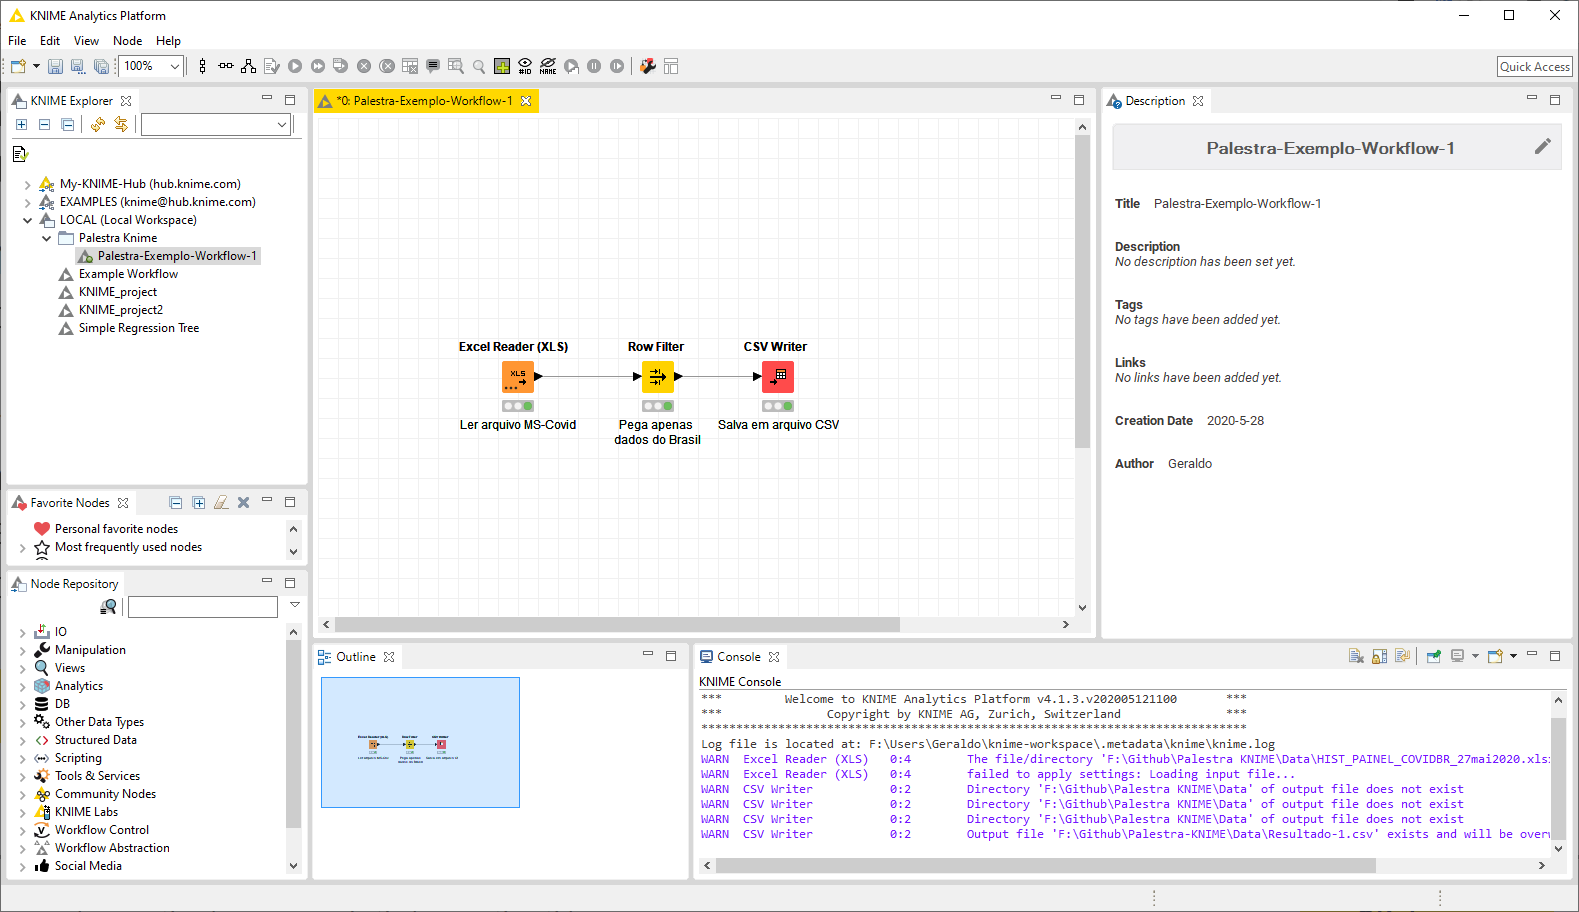
\includegraphics[width=\linewidth]{Images/Interface1}
    }

   \setlength{\TPHorizModule}{\textwidth}
   \setlength{\TPVertModule}{\textheight}

  \only<2>{
   \begin{textblock*}{30mm}(20mm,20mm)\color{white}
            Área do Workflow            
   \end{textblock*}}

  \only<3>{
    \begin{textblock*}{30mm}(-20mm,20mm)
       \color{white} Explorador            
\end{textblock*}}

  \only<4>{
    \begin{textblock*}{30mm}(-20mm,50mm)
        \color{white}Nós disponíveis            
\end{textblock*}}

  \only<5>{
    \begin{textblock*}{30mm}(60mm,20mm)
        \color{white}Descrição            
\end{textblock*}}

  \only<6>{
    \begin{textblock*}{30mm}(0mm,55mm)
       \color{white} Outline            
\end{textblock*}}

  \only<7>{
    \begin{textblock*}{30mm}(40mm,55mm)
       \color{white} Console            
    \end{textblock*}}
\end{frame}

\subsection{O que é um workflow}
\begin{frame}{O que é um workflow}
\begin{outline}
Um workflow, ou fluxo de trabalho, é uma forma de descrever uma cadeia de processamento por meio de um grafo onde nós representam processos e arestas representam o fluxo de dados entre esses processos.
\vfill
\includesvg{Images/desenho-workflow-basico-1.svg}
\end{outline}
\end{frame}


\section{Workflows}

\subsection{Entendendo um Workflow}
\begin{frame}{Entendendo um Workflow}
\begin{itemize}
    \item Um workflow é composto de nós
    \item Cada nó faz uma atividade
    \item Nós são divididos em tipos
    \item Nós tem portões de entrada e saída, de tipos diferentes
    \item Portões são conectados por fluxos, passando os dados e informações sobre eles
\end{itemize}
\vfill
\includesvg{Images/desenho-workflow-basico-1.svg}
\end{frame} 

\subsection{Entendendo um Nó}
\begin{frame}{Um nó básico}
    \begin{columns}
        \begin{column}{0.5\linewidth}
        \begin{outline}
            \1 Tipo do nó
            \1 Desenho indicativo do nó
            \1 Porta de entrada
            \1 Porta de saída
            \1 Status do nó
            \1 Nome do nó
        \end{outline}
        \end{column}
        \begin{column}{0.5\linewidth}
        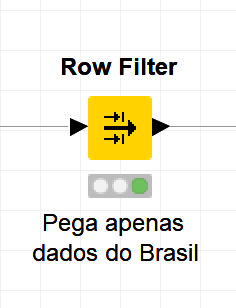
\includegraphics[width=0.8\linewidth]{Images/UmNo.png}
        \end{column}
    \end{columns}
\end{frame} 

\begin{frame}{Status do Nó}
    \begin{columns}
        \begin{column}{0.5\linewidth}
            \begin{outline}
                \1 Não configurado
                \1 Pronto para executar
                \1 Executado
            \end{outline}
        \end{column}
        \begin{column}{0.5\linewidth}
            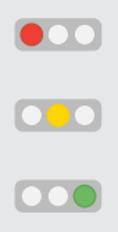
\includegraphics[height=0.8\textheight]{Images/statusdono.png}
        \end{column}
    \end{columns}
\end{frame} 


\begin{frame}{Configuração de um Nó}
    \centering
   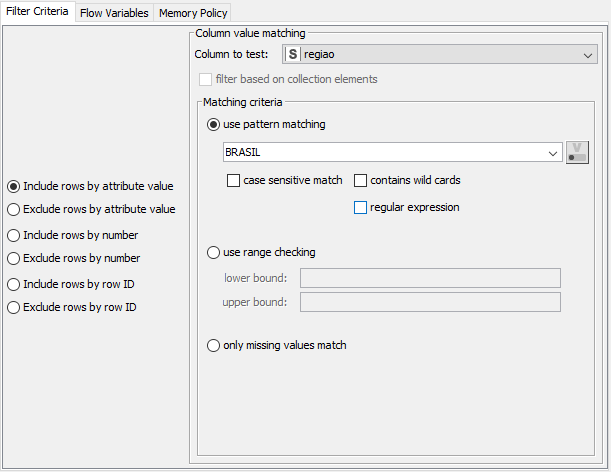
\includegraphics[width=0.8\linewidth]{Images/configuracaofiltro.png}
\end{frame} 


\subsection{Tipos de Nós}
\begin{frame}{Tipos de Nós}
    \begin{itemize}
        \item Leitura
        \item Escrita / \textit{Deploy}
        \item Transformação
        \item Análise, Aprendizado
        \item Exploração
        \item Predição
        \item Controle
    \end{itemize}
\end{frame} 

\begin{frame}{Tipos de Porta (mais comuns)}
    \centering
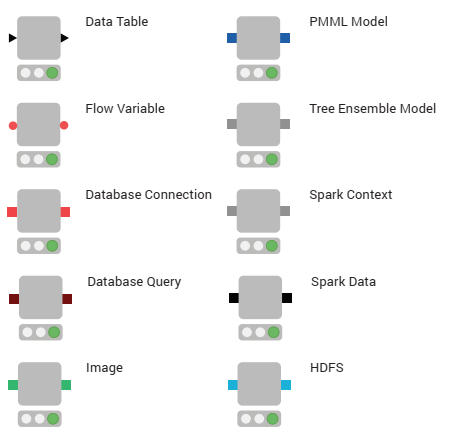
\includegraphics[width=0.8\textheight]{Images/tiposdeportas.png}    
\end{frame} 

\subsection{Construindo um Workflow}

\begin{frame}{Construindo um Workflow}
    \begin{itemize}
        \item Coloque nós no mapa
        \item Configure os nós 
        \item Execute
        \item Repita até alcançar o desejado
    \end{itemize}
\end{frame}


\section{Exemplos}

\subsection{Visualização de Curvas}
\begin{frame}{Visualização de Curvas}
    \centering
    \includesvg[width=.8\linewidth]{Images/desenha-covid-ob-ac}
\end{frame}


\subsection{Metanodes}
\begin{frame}{Metanodes}
    \centering
    \includesvg[width=.8\linewidth]{Images/metanodo}
\end{frame}

\subsection{Estudando o Covid}
\begin{frame}{Estudando o Covid-19}
    \centering
    \includesvg[width=.8\linewidth]{Images/estudaCovid.svg}
\end{frame}

\begin{frame}{Simplificando o Modelo}
    \centering
    \includesvg[width=.8\linewidth]{Images/resumido.svg}
\end{frame}


\section{BIRT -- Basic Intelligence Report Tool}

\subsection{O que é BIRT}
\begin{frame}{O que é BIRT}
Software open source usado para criar relatórios, baseado no resultado dos workflows.
Podem ser gerados em PDF, HTML e outros formatos.
\vfill
\centering
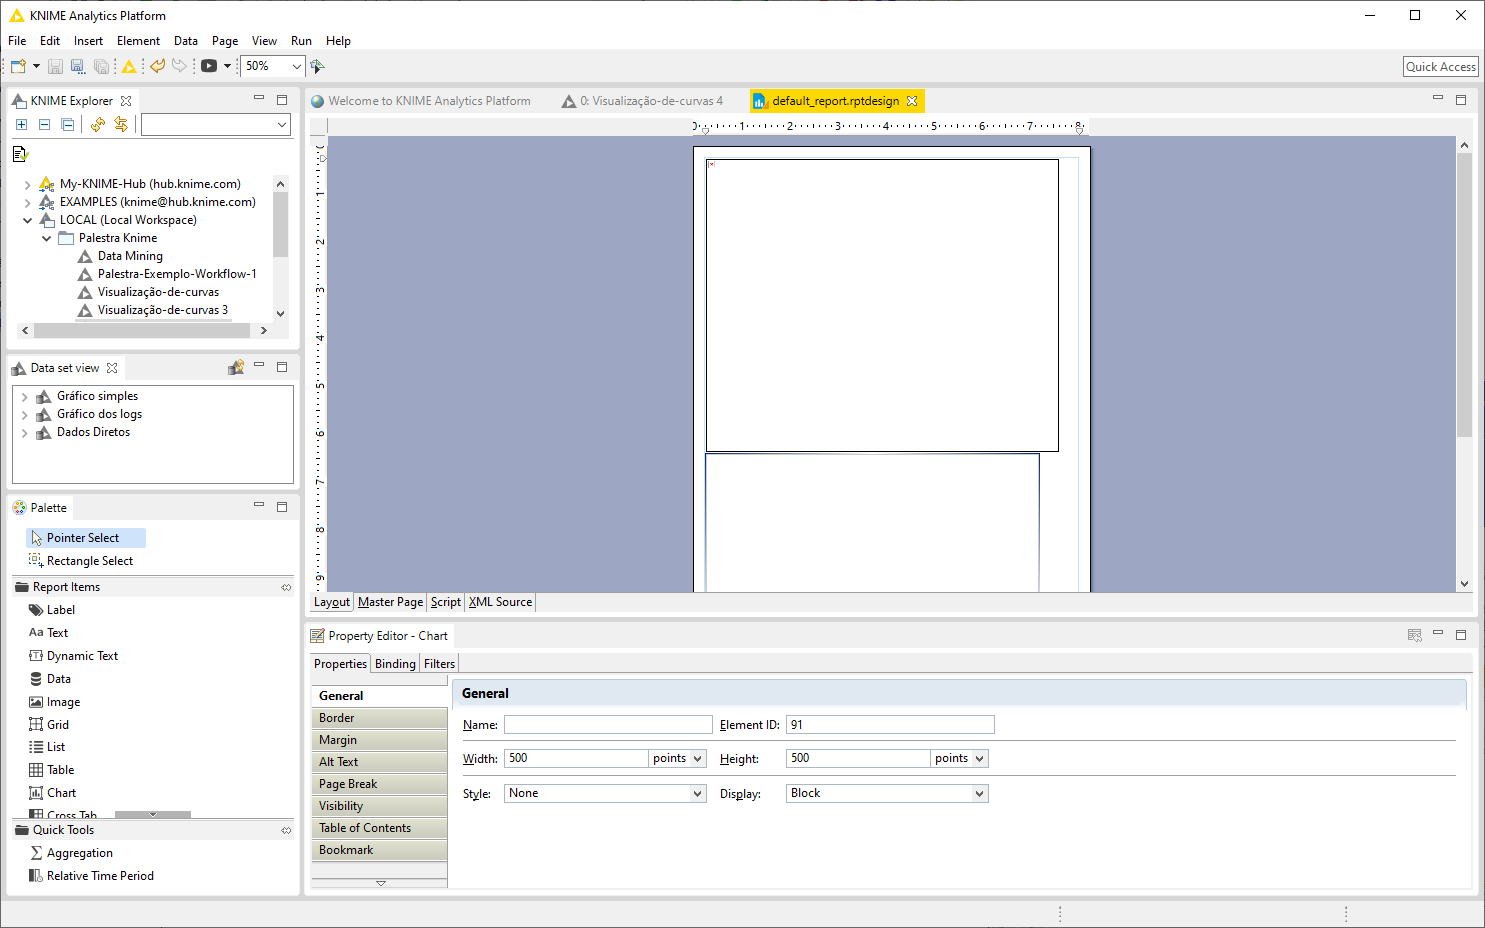
\includegraphics[height=0.4\textheight]{Images/birtscreen.png}
\end{frame} 

\subsection{Como usar BIRT}
\begin{frame}{Como usar BIRT}
    \begin{itemize}
        \item instalar (instalar plug-in no )
        \item dentro de um workflow, clicar 
\includegraphics{Images/birticon.png}
    \end{itemize}
\end{frame}

\begin{frame}{Como usar BIRT II}
    \begin{itemize}
        \item defina o layout da págica
        \item defina a master page
        \item usos mais avançados com scripts...
    \end{itemize}
\end{frame}

\begin{frame}
    \Huge \center
    Obrigado!
\end{frame} 


\begin{frame}{Contato}
    \begin{center}
        
\includegraphics[width=\linewidth]{Images/Picture5.png}
    \end{center}   
\end{frame}

\end{document}
